% Paper 10 (TN Holdings), DRAFT 1, home, 2026-11-18 (owner 20:21 JST "書いて": paper 10 is the real-time control
% paper; everything in it, nothing left for an eleventh). Built from notes/paper_ff_2026-11-17/OUTLINE.md and the
% committed records of 2026-11-16, 17 and 18 named beside each number; every number is quoted from those records
% (README and score files) and is to be checked one by one against them before release (workplace VS, as for paper 9).
% Figures: notes/paper10_ff/figures.py. The section on the updated operating layer waits for its declared device
% check (\pending). The earlier plan for a paper 10 (notes/paper10/, the cut of the 81-qubit chain) has not run.
\documentclass[10pt,a4paper]{article}
\usepackage[margin=2.2cm]{geometry}
\usepackage{amsmath,amssymb}
\usepackage{booktabs}
\usepackage{graphicx}
\usepackage[hidelinks]{hyperref}
\usepackage{url}
\setlength{\parskip}{4pt}
\setlength{\parindent}{0pt}
\sloppy
\newcommand{\pending}[1]{\textbf{[PENDING: #1]}}

\title{Decisions No Correction of the Uncontrolled Circuit Can Reach:\\ Real-Time Control on IBM Heron, Declared
Before the Data}
\author{TN Holdings\\ \small contact: \texttt{love.os.architect@proton.me}}
\date{DRAFT, 18 November 2026}

\begin{document}
\maketitle

\begin{abstract}
A circuit that measures in the middle and acts on the result at once has a natural comparison: the same circuit with
the actions removed. Whatever is done to that uncontrolled circuit after the run, including error mitigation at any
shot cost, returns at best its own noiseless value; the distance from that value to the exact answer is a
\emph{correction ceiling} $c$. We ask whether real-time control on today's cloud devices gets closer to the exact answer
than $c$, with every shot counted, no mitigation, and every test declared in git before the device record of its run
was fetched. Over three nights on three IBM Heron devices (49 declared predictions, 33 held, 16 failed and reported as
failed), chains of repeat-until-success (RUS) neurons crossed the ceiling and the margin grew with the chain length
(slope $+0.024$ per neuron on ibm\_fez; $+0.031$ and, after a recalibration, $+0.053$ for a frame-balanced pair on
ibm\_marrakesh); iterative phase estimation crossed its ceiling at $n=2,3,4$ (0.903 against 0.471 at $n=4$). Getting
there needed a diagnosis on the device: the first neuron design lost its value not to the conditionals, which cost
nothing measurable when they did not fire, but to time spent in $|1\rangle$ during mid-circuit measurement waits;
holding the likely value as $|0\rangle$ recovered 0.11--0.22. That one-sided decay can also push a design above its own
noiseless value; a guard declared beforehand took those cases out, and a frame-balanced pair removes the lean by
construction. Two limits are measured: fixed circuits can share a circuit with no loss (halving device time), but two
items with conditionals in one circuit cost the control arm (0.20 on average with ten items; 0.06 on the first of two),
which a delay did not remove and which is not explained by decisions waiting for each other (no decision latency above $\approx0.4\,\mu$s was resolved). Finally, a
prescription loop that diagnoses the device, applies a fixed rule and runs the chosen circuit ran unattended on the
device and picked a different prescription after the device was recalibrated. What the device keeps of the noiseless
value varies by night (0.61--0.87 for the same balanced pair on two nights); no quantum advantage is claimed.
\end{abstract}

\section{Introduction}\label{sec:intro}
Papers 7, 8 and 9 of this series (doi:10.5281/zenodo.24046673, 24136512, 24278888) reported raw results of fixed
circuits on IBM Heron devices through an operating layer, psf-os (doi:10.5281/zenodo.24211404), that places a circuit
from the coupling graph and the failed elements only, never reads a calibration quality number, adds its own controls to
each job and applies no mitigation. This paper turns to circuits that measure in the middle and decide what to do next
while the circuit runs (dynamic circuits, real-time control or feed-forward).

For such a circuit we always run three arms in the same job: \emph{ff} (the circuit as written, with its real-time
actions), \emph{off} (the same circuit with every conditional block removed, so the same pulses but no decision), and
\emph{floor} (the compiled ff circuit with every $X$ and $\sqrt X$ removed, so every bit is ideally 0), plus a ring
sentinel reported beside and never judged. The question is not whether ff beats off on the device (it usually does,
trivially, when off is a different computation), but whether ff gets closer to the exact answer than any correction of
off could.

\paragraph{The correction ceiling.} Error mitigation estimates the noiseless value of the circuit that was run. For the
off arm that value, $P_\mathrm{off}^{(0)}$, is fixed by the circuit; however many shots a correction uses, it returns at
best $P_\mathrm{off}^{(0)}$. We call $c = |P_\mathrm{off}^{(0)} - \text{exact}|$ the correction ceiling and say ff is
\emph{beyond the correction ceiling} when $g = c - |P_\mathrm{ff} - \text{exact}| \ge 2\,\mathrm{SE}$. For teleportation
and phase estimation, where the off arm's bits can be decoded shot by shot, the ceiling is the best such decoder's
noiseless value (3/4 for one-bit teleportation by the best fixed rule; the Bayes-best decoder for phase estimation). Two
scope statements matter. First, this is not a claim that dynamic circuits cannot be mitigated: probabilistic error
cancellation has been extended to mid-circuit measurement and feed-forward (Gupta et al.\ 2023); the ceiling concerns
correcting the circuit \emph{without} the control. Second, writing the control coherently, without mid-circuit
measurement, gives the same noiseless answer and can be corrected afterwards (section~\ref{sec:coherent}); the claim is
about what correction of the uncontrolled circuit can reach, not about every possible circuit. The ceiling also differs
from the known limits of mitigation (Takagi et al.\ 2022; Quek et al.\ 2024), which bound its shot cost; ours is a
bound on its aim.

\paragraph{Prior work.} RUS neurons (Cao, Guerreschi, Aspuru-Guzik 2017) have run with real-time feedback on a
superconducting processor as a three-neuron network (Moreira et al.\ 2023), and iterative phase estimation with dynamic
circuits on IBM devices (C\'orcoles et al.\ 2021); constant-depth long-range entanglement with dynamic circuits was
compared with unitary circuits by B\"aumer et al.\ (2023). Real-time correction beyond break-even (Sivak et al.\ 2023;
Google Quantum AI 2024) is the closest idea to the ceiling, in a very different setting. What is new here is the
yardstick (a ceiling against correction of the uncontrolled circuit), chains up to seven neurons on cloud devices with
every shot counted and no mitigation, the device diagnosis that made the chains work, the measured limits of packing and
timing, and a declared prescription loop.

\section{Method}\label{sec:method}
\paragraph{Declaration.} Every test was written as a declaration (\texttt{prereg/} in the lab notebook) with its tools,
verdict words and predictions, committed and pushed to git before the device record of its run was fetched; the tools
as of the declaring commit are the verdict tools. A prediction holds or fails as a whole and a failed one is reported
as failed. The device is chosen by a standing rule from the queue (the first qualifying of ibm\_marrakesh, ibm\_fez,
ibm\_kingston); placement uses the coupling graph and the failed marks only. Dynamical decoupling and twirling are off,
no mitigation is applied, 4000 shots per circuit unless stated, and every shot is counted (post-selection appears only
beside a verdict). A pre-run check simulates every arm of the built job without noise and compares it with its
noiseless value; a failed check means the job is not submitted. Each job returned byte-identical to the one built, and
every result re-scores from its committed raw counts (\texttt{reproduce.py}).

\paragraph{Verdicts.} CLOSER WITH CONTROL: $d = |P_\mathrm{off} - \text{exact}| - |P_\mathrm{ff} - \text{exact}|
\ge 2\,\mathrm{SE}_d$ on the device. BEYOND THE CORRECTION CEILING as above. OVERSHOOT: $P_\mathrm{ff}$ above its own
noiseless value by more than 2 SE; an overshooting point is never credited as beyond (section~\ref{sec:decay}).
COMPOUNDS: the slope of $g$ over the chain length is at least 2 SE and no point overshoots.

\paragraph{The neuron chain.} A RUS neuron at $\theta = 1.1$ maps its input to $P_1 = \sin^2 q$ with $\tan q = \tan^2
\theta$; a chain of $L$ neurons gives $(\sin^2 q)^L$ exactly (0.937, 0.878, 0.823, \dots, $L = 1, 2, 3$). Each neuron
tries up to $m$ times; after a failed try the conditional block undoes the rotation on the output. With $m = 2$ the
noiseless value of the chain lies below the exact value by the share of shots still failing after two tries (0.892,
0.793, 0.706, 0.629, 0.560 against 0.937, 0.878, 0.823, 0.771, 0.723 for $L = 1..5$): this is the design's own cost and
is reported separately. The off arm's noiseless values give the ceiling $c(L) = 0.143, 0.247, 0.322, 0.373, 0.407,
0.426, 0.435$ for $L = 1..7$.

\section{Making the neuron chain work: a diagnosis on the device}\label{sec:diagnosis}
\paragraph{First design (11-16, marrakesh).} The control fired as the circuit says (the try patterns of the first
neuron matched their noiseless shares within 0.012), but the value was lost: ff 0.599, 0.629, 0.551 at $L = 1, 2, 3$
against noiseless 0.918, 0.850, 0.790, and not closer than off at $L = 1, 2$ (two of three predictions failed;
\texttt{results/rus-neuron-2026-11-16}).

\paragraph{What it was not, and what it was.} A wait diagnostic placed an output next to mid-circuit measurements with
and without conditionals that never fire: the unfired conditionals cost $+0.006$ (2 SE 0.022), nothing measurable (the
declared prediction that they would cost failed), while the measurements beside an output in $|1\rangle$ cost it 0.23 on
physical qubit 1 (\texttt{wait-diag-2026-11-16}). A control diagnostic then held a $|1\rangle$ through five
mid-circuit measurements before using it as a control: on qubit 1 its value as a control fell from 0.98 to 0.46, on
qubit 3 from 0.96 to 0.72, and measuring neighbours instead of a far qubit added nothing beyond 2 SE
(\texttt{ctrl-diag-2026-11-16}). The loss is time spent in $|1\rangle$ during measurement waits, toward $|0\rangle$,
which decoupling does not undo; every retry adds waits, and the off arm, making one attempt, waits less.

\paragraph{Designs 2 and 3.} Holding every output whose likely value is 1 flipped (as $|0\rangle$) around each
measurement, with barriers so the compiler keeps the flips, moved ff toward the exact value by $+0.113$, $+0.179$,
$+0.182$ at $L = 1, 2, 3$ (2 SE 0.021--0.022; \texttt{rus-neuron2-2026-11-16}). Reading the last output flipped as
well (the third design) added $+0.217$ at $L = 1$, where the output qubit read $|1\rangle$ as 1 in only about 0.8 of the
shots; ff then stood at 0.883, 0.740, 0.631 against the design's noiseless 0.892, 0.792, 0.708, CLOSER at every $L$
(\texttt{rus-neuron3-2026-11-16}). The same circuits on ibm\_kingston gave 0.853, 0.749, 0.646, CLOSER at every $L$
(\texttt{rus-neuron3-kingston-2026-11-16}).

\section{Beyond the correction ceiling, and a margin that grows}\label{sec:beyond}
Figure~\ref{fig:ceiling} collects the chains.

\begin{figure}[t]
\centering
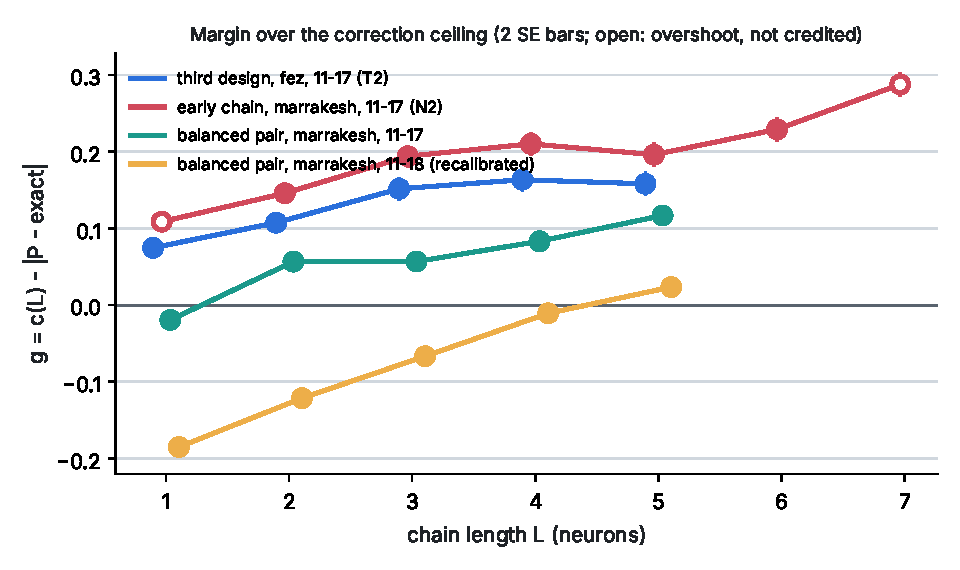
\includegraphics[width=0.78\linewidth]{fig_ceiling.pdf}
\caption{Margin $g = c(L) - |P - \text{exact}|$ over the correction ceiling against the chain length, with 2 SE bars.
Filled: credited points; open: overshoot (above the design's own noiseless value), not credited. Blue: third design on
ibm\_fez (11-17, T2). Red: early-measured chain on ibm\_marrakesh (11-17, N2). Green and yellow: the frame-balanced
pair on ibm\_marrakesh on 11-17 and on 11-18 after the device was recalibrated.}
\label{fig:ceiling}
\end{figure}

\paragraph{Third design on ibm\_fez (11-17, T2).} Beyond the ceiling at every $L = 1..5$ ($g = +0.075, +0.107, +0.152,
+0.164, +0.158$, 2 SE 0.011--0.016), no overshoot, slope $+0.024$ per neuron (2 SE 0.004): COMPOUNDS. Against its own
noiseless value ff was $-0.021$ to $-0.086$: the device kept 0.65--0.78 of the noiseless margin, and the growth slowed at
$L = 4, 5$ (\texttt{results/ff-night-2026-11-17/compound}). An early-measured form of the chain (10 CZ against 42 at
$L = 5$, a third of the counted waits) gave the same within 2 SE at every $L$ (T4; the prediction that it would keep more
failed): neither the CZ count nor the counted waits limited the chain on that night.

\paragraph{Early chain to seven neurons (11-17, marrakesh, N2).} Beyond the ceiling at $L = 2..6$ ($g$ up to $+0.229$),
but above its own noiseless value at $L = 1$ (0.903 against 0.890) and $L = 7$ (0.487 against 0.444); the declared
guard took those points out and the slope is NOT SHOWN (both predictions failed;
\texttt{results/ff-night2-2026-11-17}).

\paragraph{The frame-balanced pair (11-17 and 11-18, marrakesh).} Section~\ref{sec:decay} explains the pair. On 11-17 it
did not overshoot anywhere, was beyond the ceiling at $L = 2..5$ ($g = +0.057$ to $+0.117$) but not at $L = 1$
($-0.019$), and compounded ($+0.031$ per neuron, 2 SE 0.003). The same job on the same device and qubits on 11-18, after
the device had been recalibrated that morning, again did not overshoot and compounded faster ($+0.053$, 2 SE 0.003),
but was beyond only at $L = 5$ ($g = -0.185, -0.121, -0.067, -0.011, +0.024$): the pool kept 0.61--0.68 of its noiseless
value against 0.77--0.87 the night before. Its growth on 11-18 comes from the ceiling rising with $L$ faster than the
device lost, not from the device keeping more (\texttt{balanced-night-2026-11-17}, \texttt{balanced-repeat-2026-11-18};
the repeat's prediction ``beyond at $L = 2..5$'' failed).

\paragraph{Phase estimation and teleportation.} Iterative phase estimation (C\'orcoles et al.\ 2021) was beyond its
Bayes-decoder ceiling at $n = 2$ (0.861 against 0.750) and $n = 3$ (0.772 against 0.588) on ibm\_fez with a growing
margin, and at $n = 4$ on ibm\_marrakesh, pooled over its 16 phases, 0.903 (2 SE 0.002) against 0.471. One-bit
teleportation was above the best fixed rule's 3/4 on 11-16 (0.952 and 0.890 at $k = 1, 2$; marrakesh) and, written so
that decay works against success, at $k = 2$ (0.849) but not $k = 4$ (0.734) on ibm\_fez (that prediction failed).

\paragraph{Two numbers.} Beyond the ceiling with a margin that grows with depth, on two devices and again on a second
night. And what the device keeps varies by night and device more than by design: 0.65--0.78 of the noiseless margin for
the third design on fez, and for the same balanced pair on the same qubits 0.77--0.87 of the noiseless value on 11-17
against 0.61--0.68 on 11-18, after a recalibration.

\section{One-sided decay, overshoot and the frame-balanced pair}\label{sec:decay}
Decay during waits and on readout moves $|1\rangle$ to $|0\rangle$ only. A design that holds the likely value 1 as
$|0\rangle$ (the third design) turns this one-sided decay into a lift toward success and can read above its own
noiseless value. We saw it at $L = 1$ and 7 of the early chain and at $L = 1$ of the prescription loop
(section~\ref{sec:loop}); the off arms of the read-flipped designs also often read above their noiseless values. A
closeness to the exact value that comes from decay is not the control's doing, so every such point is excluded by a
guard written before the data.

The frame-balanced pair runs each $L$ in two complementary frames in one job: rd (the third design: logical 1 waits and is
read as $|0\rangle$) and nf (the same barriers and waits, no flips: logical 1 waits and is read as $|1\rangle$), and is
judged on $P = (P_\mathrm{rd} + P_\mathrm{nf})/2$. In each frame every logical value spends the same time as $|1\rangle$,
so one-sided decay acts on the pool as a symmetric flip, which pulls toward 1/2 and cannot lift $P$ above a noiseless
value above 1/2. On the device the pool never overshot. The price is visible in the two frames: on 11-17 rd kept
0.92--1.01 and nf 0.60--0.80 of the noiseless value; nf at $L = 1$ read its 1 on a qubit whose $|1\rangle$ read as 1 in
0.83 of the shots. After the 11-18 recalibration that qubit's readout gap had reversed (0.967 for $|1\rangle$ against
0.955 for $|0\rangle$), and it was rd that lost on readout.

\section{Without mid-circuit measurement}\label{sec:coherent}
The same neuron written coherently (no mid-circuit measurement, the control as controlled gates) was CLOSER WITH CONTROL
at $L = 1$ on ibm\_fez and at $L = 2, 3$ on ibm\_marrakesh (11-17, T1 and N1). On fez at $L = 1$ it was 0.032 further from
its noiseless value than the measured third design (8 CZ against 2 CZ and two measurements); on marrakesh at $L = 2, 3$ the
two kept the same within 2 SE. The coherent form has the same noiseless value as ff and can be corrected afterwards, so
it marks where our claim stops (section~\ref{sec:intro}).

\section{A prescription loop, and running it unattended}\label{sec:loop}
\paragraph{The loop (11-17, marrakesh).} A fixed list of prescriptions (P0 the circuit as written; P1 hold flipped while
waiting; P2 P1 and read flipped; P3 fewer tries) and a fixed rule read only the night's own diagnostics: a late-use loss
in the control diagnostic gives P1; with a readout gap on the output qubit, P2; else an unfired-conditional cost gives P3;
else P0. On 11-17 the rule picked P2 at $L = 1, 2, 3$; the prescription helped at $L = 2, 3$ ($+0.043$, $+0.079$ against
the circuit as written) and overshot at $L = 1$ (one of two predictions failed; \texttt{results/os-night-2026-11-17}).

\paragraph{Compounding loop, first device night (11-18, marrakesh).} The loop was extended to rounds: each round's result
is the next round's input, prescriptions stack in a fixed order (base, +B the balanced pair, +Q move the output to a qubit
with less readout gap), and a loss-cutting rule removes the last step after two rounds without a credited gain; a fixed
point, four rounds or 240 s of device time by the model stop it. On 11-18 one command on the owner's machine ran it with
nobody in between: diagnostics showed a late-use loss but no readout gap on the output qubits (the device had been
recalibrated at 10:40), so the rule picked P1, not the previous night's P2; P1 helped at every $L$ ($+0.032, +0.026,
+0.055$, 2 SE 0.017--0.022) without overshoot; the rule kept every stack and the loop stopped at a fixed point after one
round (82 s charged). The prediction that the rule would change a stack between rounds failed; the one that the last
round would not overshoot held. A check of the run on the owner's machine and at home gave the same scores, rules and
stop (\texttt{results/os2-night-2026-11-18}). The loop reads no calibration error numbers; that, and choosing only among
declared entries, distinguish it from automatic calibration graphs that read them (Kelly et al.\ 2018).

\section{Limits: packing and timing}\label{sec:limits-pack}
\begin{figure}[t]
\centering
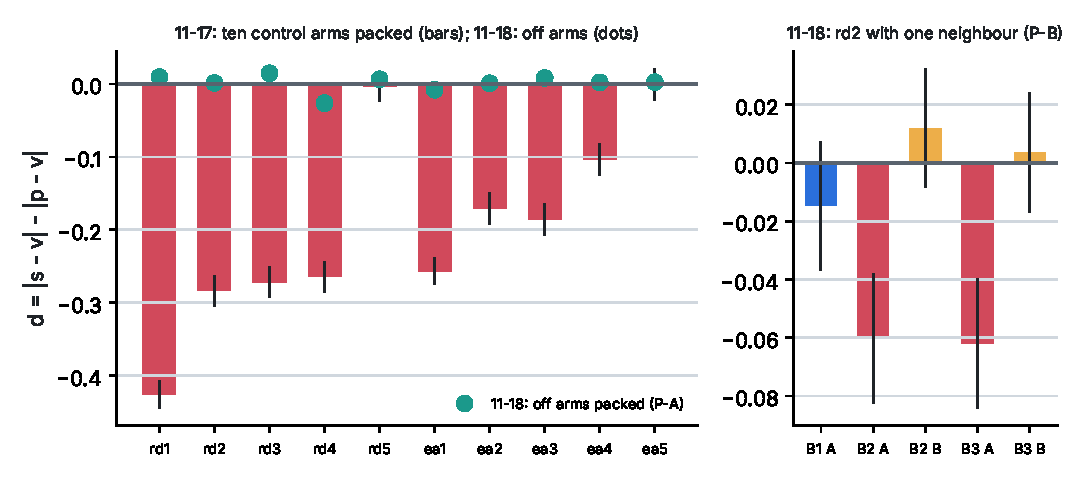
\includegraphics[width=\linewidth]{fig_packing.pdf}
\caption{Left: packed against alone on the same qubits, $d = |s - v| - |p - v|$ (negative: packed kept less). Bars:
ten items' control arms packed into one circuit per arm (11-17); dots: the same items' off arms packed (11-18, P-A).
Right: rd2 with one neighbour (11-18, P-B): B1 neighbour without conditionals; B2 both with conditionals; B3 as B2 with
the second item delayed past the first's whole duration as written. 2 SE bars.}
\label{fig:packing}
\end{figure}

\paragraph{Packing.} Running ten independent items side by side in one circuit per arm cut the device time from 41 s to
11 s, but the control arm kept 0.20 less on average (2 SE 0.007; up to 0.43), while the off arm agreed within 0.03
(11-17, \texttt{packing-night-2026-11-17}). On 11-18 the off arms of the same items packed into one circuit read as they
read alone (mean $d = +0.001$, 2 SE 0.007; P-A): a production form with the control arms alone and only the fixed
circuits packed needs 16 circuits and 20.9 s by the model against 34 circuits and 40.9 s, with the same CLOSER verdicts.
With rd2 and one neighbour (P-B), a neighbour without conditionals cost nothing beyond 2 SE ($-0.015$); a neighbour with
conditionals cost the first item 0.060 and left the second unchanged ($+0.012$); delaying the second item past the first's
whole duration, as written, left the same loss on the first ($-0.062$; the prediction that the delay would remove it
failed). An independent re-reading confirmed that the loss sits on the first item's output bit
(\texttt{parallel-night-2026-11-18}). None of the blocks qualifies for the controller's low-latency path (each holds a
CZ).

\paragraph{Timing.} Clock qubits on a ruler of delays read a mid-circuit measurement step as 2.78\,$\mu$s; a fast-path
decision added $+0.32\,\mu$s (2 SE 0.42), NOT RESOLVED (the prediction that it would be resolved failed); two
fast-path actors and two actors whose blocks hold a CZ each ran side by side, ratios 0.96 (2 SE 0.19) and 1.00 (2 SE 0.22)
(the prediction that the CZ actors would wait for each other failed; \texttt{timing-night-2026-11-18}). So the packing
loss is not explained by decisions waiting for each other at this resolution; its mechanism is open.

\section{What did not hold}\label{sec:failed}
\begin{table}[h]
\centering\small
\begin{tabular}{@{}lll@{}}
\toprule
night & prediction & what happened \\
\midrule
11-16 & teleport: off arm at or under its circuit value & decay toward the success bit lifted the off arm \\
11-16 & neuron, first design, CLOSER at $L = 1, 2$ & value lost in measurement waits (section~\ref{sec:diagnosis}) \\
11-16 & wait: unfired conditionals cost & they cost nothing measurable \\
11-17 & teleport $k = 4$ beyond 3/4 & 0.734 \\
11-17 & early chain keeps more than the third design & the same within 2 SE \\
11-17 & early chain to $L = 7$: beyond at every $L$; compounds & overshoot at $L = 1, 7$ \\
11-17 & loop: prescription helps at $L = 1, 2, 3$ & overshoot at $L = 1$ \\
11-17 & balanced pair beyond at every $L$ & not at $L = 1$ (readout gap of qubit 1) \\
11-17 & packing keeps the same & control arm $-0.20$ \\
11-18 & balanced repeat beyond at $L = 2..5$ & only at $L = 5$ after the recalibration \\
11-18 & a delay removes the packing loss & it did not \\
11-18 & fast-path decision latency resolved & $+0.32 \pm 0.42\,\mu$s (2 SE) \\
11-18 & CZ actors wait for each other & ratio 1.00 \\
11-18 & compounding loop changes a stack & fixed point after round 1 \\
\bottomrule
\end{tabular}
\caption{The 16 failed predictions of 49 (the early-chain row counts two; the 11-16 neuron row counts two).}
\end{table}

\section{Limits}\label{sec:limits}
\begin{itemize}
\item Three devices, three nights, mostly one device per test; the same-device repeat on 11-18 followed a recalibration and
kept much less. What the device keeps varies by night more than by design.
\item The ring sentinel was DEAD on marrakesh and fez on most of these nights; it is reported and never judged.
\item The ceiling is defined against correction of the uncontrolled circuit, as declared; post-selection (discarding
shots) is not a correction in this sense and is reported only beside.
\item The neuron's exact value is that of the intended neuron (unbounded tries); with $m = 2$ the noiseless design lies
0.04--0.19 below it ($L = 1..7$), which the device can never recover.
\item Every noise model in the notes is illustrative and not fitted; none is used for a verdict.
\item A sentinel's compiled bytes depend on the qiskit-aer version; user, off and floor circuits rebuilt byte-identical
across machines.
\end{itemize}

\section{The updated operating layer}\label{sec:update}
\pending{psf-os v0.2.0: real-time control entrance (explicit off arm, packed items, given placement, top-level delay,
register conditions), build rules from sections~\ref{sec:loop}--\ref{sec:limits-pack} (fixed circuits packed
automatically; no two conditional items in one circuit; the build environment recorded), the compounding loop in the
package, the frame chosen from each output qubit's readout; and its declared device check of 2026-11-19.}

\section{Reproduction}\label{sec:repro}
Every device result re-scores from its committed raw counts with \texttt{python reproduce.py} in
\texttt{psf-os-lab-notebook} with psf-os at the commit named in each folder (\texttt{feedforward-2026-11-16}); the
entries of 11-16 to 11-18 re-scored the same on 2026-11-18, and an independent re-reading with qiskit and numpy only
(\texttt{notes/verify\_2026-11-18}) gave the same numbers and verdicts for 11-18. Figures:
\texttt{notes/paper10\_ff/figures.py}.

\section{Conclusion}
Real-time control on cloud IBM Heron devices got closer to the exact answer than any correction of the uncontrolled
circuit could, declared before the data with every shot counted, and for chains of neurons the margin grew with the chain
length, on two devices and on a second night. It took a diagnosis on the device: the conditionals were free, the waits
were not, and where a value waits decided how much of it survived. The same one-sided decay that the fix exploits can
fake closeness, which a declared guard and a frame-balanced pair keep out of the verdicts. Fixed circuits can share a
circuit for free, conditional ones cannot yet, for a reason the timing does not show. And a loop that reads the night's
own diagnostics and nothing else chose a different prescription when the device changed.

\section*{Data and code}
Records, declarations and raw counts: \url{https://github.com/TN-Holdings-LLC/psf-os-lab-notebook}; the operating
layer: \url{https://github.com/TN-Holdings-LLC/psf-os} (doi:10.5281/zenodo.24211404; branches
\texttt{feedforward-2026-11-16}, \texttt{register-cond-2026-11-18}).

\section*{References}
\begin{itemize}
\item Cao, Y., Guerreschi, G.\ G., Aspuru-Guzik, A. Quantum neuron: an elementary building block for machine learning on
quantum computers. arXiv:1711.11240 (2017).
\item Moreira et al. Realization of a quantum neural network using repeat-until-success circuits in a
superconducting quantum processor. npj Quantum Information 9, 118 (2023).
\item Gupta et al. Probabilistic error cancellation for dynamic quantum circuits. arXiv:2310.07825 (2023).
\item Takagi, R., Endo, S., Minagawa, S., Gu, M. Fundamental limits of quantum error mitigation. npj Quantum Information 8,
114 (2022); arXiv:2109.04457.
\item Quek, Y.\ et al. Exponentially tighter bounds on limitations of quantum error mitigation. Nature Physics;
arXiv:2210.11505.
\item C\'orcoles, A.\ D.\ et al. Exploiting dynamic quantum circuits in a quantum algorithm with superconducting qubits.
Phys.\ Rev.\ Lett.\ 127, 100501 (2021).
\item B\"aumer, E.\ et al. Efficient long-range entanglement using dynamic circuits. arXiv:2308.13065 (2023).
\item Sivak, V.\ V.\ et al. Real-time quantum error correction beyond break-even. Nature 616, 50--55 (2023).
\item Google Quantum AI. Quantum error correction below the surface code threshold. arXiv:2408.13687 (2024).
\item Kelly, J.\ et al. Physical qubit calibration on a directed acyclic graph. arXiv:1803.03226 (2018).
\item TN Holdings. Papers 7, 8 and 9 of this series: doi:10.5281/zenodo.24046673, 24136512, 24278888.
\end{itemize}

\end{document}
